
This Chapter returns to the 2D Poisson equation last seen in Chapter \ref{chap:st}.  Here we implement a finite element method (FEM) for an unstructured triangular mesh covering a general domain.  Our approach is to first
\begin{center}
\emph{do element-wise assembly of the residual equations,}
\end{center}
and thereby get a functioning, \pSNES-using code without even thinking about matrices as we write code.  Only after making sure it works do we write additional code to assemble the Jacobian matrix.  Our code will solve certain nonlinear Poisson equations in addition to the linear case.

We use \PETSc for some new tasks:
\begin{itemize}
\item reading a triangular mesh from a file into \PETSc \pVecs,
\item managing unstructured indexing of that mesh, and
\item implementing Neumann boundary conditions.
\end{itemize}

The FEM here contrasts with the structured rectangular-element ($Q^1$) FEM of Chapter \ref{chap:of} in that it does not use \PETSc's \pDMDA or other mesh-topology infrastructure.  As a consequence, our implementation work-load increases substantially.  We both find out what we lose by not using \pDMDA, and we understand better what mesh-topology and indexing tools in \PETSc are doing.

On the other hand, this example is representative of \PETSc applications where direct contact with file formats and index sets is required.  We use the relatively-simple \texttt{triangle} program, and it generates ASCII files describing the mesh.  Our code uses a new-to-us \PETSc \pIS type for managing the indexing of nodes and triangles.  In Chapter \ref{chap:dp} we will return to unstructured FEM methods, and there take advantage of \PETSc's \pDMPlex class for some of the unstructured mesh tasks done ``by-hand'' here.

The residual equations are the FEM discretizion of the weak form of the PDE.  Our direct construction of these equations roughly follows the residual implementation of the $p$-Laplacian equation in Chapter \ref{chap:of}.  However, the well-known stiffness matrix ``$A$'', and corresponding linear system ``$A\bx = \bb$,'' the major pieces of the standard construction in FEM introductions \citep{Braess2007,Elmanetal2005}, arise here as the Jacobian, and Newton step, respectively, when solving our residual equations.  As noted, in our first runs, done before writing Jacobian-assembling user code, we allow \PETSc \pSNES to handle all the details of this linear-system-construction by using finite-differencing and residual evaluations.

\section{A 2D nonlinear Poisson problem}

\begin{marginfigure}
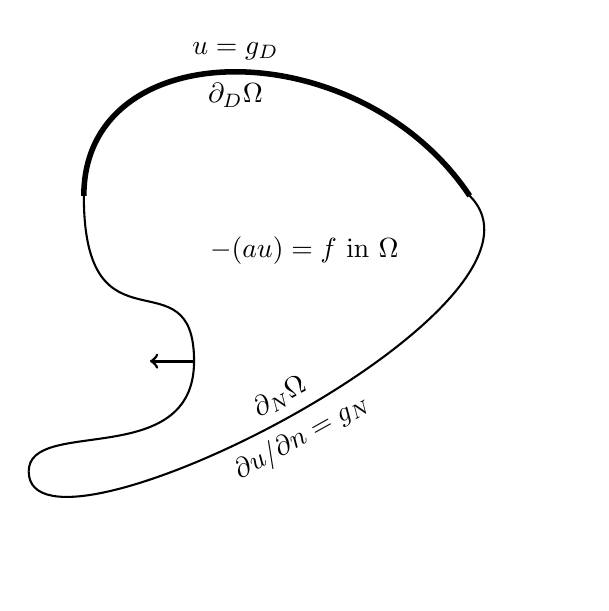
\begin{tikzpicture}[scale=0.7]
%\draw[gray,very thin] (-2,-6) grid (8,3);
\draw[line width=2pt] (0,0) .. controls (0,3) and (5,3) .. node[sloped,above] {$u=g_D$} node[sloped,below] {$\partial_D\Omega$} (7,0);
\draw[line width=0.75pt] (7,0) .. controls (9,-2) and (-1,-7) .. node[sloped,above] {$\partial_N\Omega$} node[sloped,below] {$\partial u/\partial n = g_N$} (-1,-5);
\draw[line width=0.75pt] (-1,-5) .. controls (-1,-4) and (2,-5) .. (2,-3);
\draw[line width=0.75pt] (2,-3) .. controls (2,-1) and (0,-3) .. (0,0);
\draw[->,line width=1.0pt] (2,-3) -- (1.2,-3) node[below] {$\bn$}; % normal vector
\draw (4,-1) node {$- \Div (a \grad u) = f$ in $\Omega$};
\end{tikzpicture}


\caption{Problem \eqref{eq:un:poissonstrong} on a domain.}
\label{fig:un:generalpoissondomain}
\end{marginfigure}

Let $\Omega \subset \RR^2$ be a bounded (open) region.  Suppose its boundary $\partial\Omega$ is well-behaved (polygonal or Lipschitz-continuous \citep[section 1.2]{Ciarlet2002}).  Suppose $\partial\Omega$ is decomposed into (measurable) disjoint subsets $\partial_D \Omega$ and $\partial_N \Omega$ whose union is the entire boundary $\partial \Omega$.

The strong form of the Poisson problem (Chapter \ref{chap:st}) includes the equation 
    $$- \grad^2 u = f \quad \text{ on } \Omega.$$
We allow a somewhat more general nonlinear form.  Let $a(x,y,u)$ and $f(x,y,u)$ be continuous functions for which there is $\eps>0$ so that
    $$a(x,y,u) \ge \eps > 0,$$
so that we require \emph{uniform ellipticity}.  The strong form should also include boundary conditions, and we will allow nonhomogeneous Dirichlet and Neumann boundary conditions.  Thus the  \emph{nonlinear-Poisson (nonlinear-diffusion) strong form} we solve is to find $u(x,y)$ so that
\begin{align}
- \Div \left(a(x,y,u) \grad u\right) &= f(x,y,u) \quad \text{ on } \Omega, \label{eq:un:poissonstrong} \\
u &= g_D \quad \text{ on } \partial_D \Omega, \notag \\
\frac{\partial u}{\partial n} &= g_N \quad \text{ on } \partial_N \Omega. \notag
\end{align}
By definition, $\partial u/\partial n = \bn \cdot \grad u$ where $\bn$ is the outward unit normal on $\partial \Omega$.

The data of problem \eqref{eq:un:poissonstrong}, besides the region $\Omega$ and its boundary, includes a \emph{diffusion coefficient} $a$, a \emph{source term} $f$, \emph{Dirichlet data} $g_D$, and \emph{Neumann data} $g_N$.  (For the purpose of numerical solutions we will simply assume that the latter boundary data is continuous.)  Poisson problem \eqref{poissonsquare} in Chapter \ref{chap:st} is the homogeneous Dirichlet case where $\Omega$ is the square, $a\equiv 1$, $f=f(x,y)$ is independent of the solution $u$, $\partial_D \Omega = \partial \Omega$, $\partial_N \Omega = \emptyset$, and $g=0$.

Problem \eqref{eq:un:poissonstrong} is not the most general (nonlinear) Poisson problem because, specifically, one could require boundary conditions which combine the above with coefficients, e.g.~``$\alpha u + \beta \frac{\partial u}{\partial n} = \gamma$ where, generally, $\alpha,\beta,\gamma$ could vary along the boundary \citep{Elmanetal2005}.  One could also allow $a$ and $f$ to depend on the gradient of $u$, as does $a=|\grad u|^{p-2}$ in the $p$-Laplacian equation of Chapter \ref{chap:of}.

As \eqref{eq:un:poissonstrong} is stated there may be no solution where ``$\Div(a\grad u)$'' makes sense as a continuous function, even for polygonal regions and continuous data.  There may be no $u\in C^2(\Omega) \cap C(\overline \Omega)$ so that $-\Div(a\grad u) = f$.  There is, however, a solution in the linear case, at least, if we convert \eqref{eq:un:poissonstrong} to a \emph{weak form}.

A weak formulation arose in Chapter \ref{chap:of} as the gradient of an objective function.  Here we will derive it from the strong form in the traditional way, by multiplying by a test function and integrating.

\section{Weak form with general boundary values}

Recall $L^2(\Omega)$ is the space of all square-integrable real functions on $\Omega$.  Define the following Sobolev space \citep{Evans2010} which is also a Hilbert space:
    $$H^1(\Omega) = \left\{u \,:\, u \in L^2(\Omega) \,\&\, \grad u \in L^2(\Omega)\right\}.$$
Definition \eqref{eq:of:sobolevdefn} of $W^{1,p}(\Omega)$ says $H^1(\Omega) = W^{1,2}(\Omega)$, but this Chapter uses the alternate notation with ``$H$'' for ``Hilbert.''

We use two subsets of $H^1(\Omega)$: \emph{trial functions} come from $H_{g}^1(\Omega)$, which denotes the functions with value $g_D$ along $\partial_D \Omega$, and \emph{test functions} come from $H_{0}^1(\Omega)$, with value $0$ along $\partial_D \Omega$.  Note that $H_{0}^1(\Omega)$ is a linear subspace of $H^1(\Omega)$ while generally $H_{g}^1(\Omega)$ is not.

To weakly-formulate the Poisson problem we choose any $v\in H_{0}^1(\Omega)$, multiply the first equation in \eqref{eq:un:poissonstrong} by $v$, and integrate by parts:
\begin{equation*}
\int_\Omega a(u) \grad u \cdot \grad v - \int_{\partial\Omega} \frac{\partial u}{\partial n} v = \int_\Omega f(u) v.
\end{equation*}
In writing weak forms we will generally suppress dependence on $x,y$ but show dependence on the solution $u$, so $a(x,y,u)=a(u)$ and similarly for $f$.

Next we use the boundary information, namely that $v=0$ on $\partial_D\Omega$ and $\frac{\partial u}{\partial n}=g_N$ on $\partial_N\Omega$:
\begin{equation}
\int_\Omega a(u) \grad u \cdot \grad v = \int_\Omega f(u) v + \int_{\partial_N\Omega} g_N v\quad \text{ for any } v\in H_{0}^1(\Omega). \label{eq:un:poissonweak}
\end{equation}
Equation \eqref{eq:un:poissonweak} is the \emph{weak formulation} of \eqref{eq:un:poissonstrong}, and any $u \in H_{g}^1(\Omega)$ satisfying it is a \emph{weak solution}.  A key observation is that Dirichlet boundary conditions are incorporated into defining $H_{g}^1(\Omega)$.  By contrast, both the Neumann boundary data $g_N$ and the source function $f$ explicitly appear in the weak form \eqref{eq:un:poissonweak}.

The rules for passing between the strong \eqref{eq:un:poissonstrong} and weak \eqref{eq:un:poissonweak} formulations clarify the situation:\begin{itemize}
\item A well-behaved function $u \in C^2(\Omega) \cap C(\overline \Omega)$ which satisfies the strong form also solves the weak form.\sidenote{The derivation above shows this.}
\item If $u \in H_{g}^1(\Omega)$ solves the weak form then we accept it, by definition, as a solution.   If it is also well-behaved (i.e.~$u \in C^2(\Omega) \cap C(\overline \Omega)$) then we may reverse the derivation to show it solves the strong form.
\end{itemize}

Consider the linear case where $a(x,y)$ and $f(x,y)$ are independent of $u$.  If $\partial_D \Omega$ has positive size, in an appropriate sense, then a solution to weak formulation \eqref{eq:un:poissonweak} exists and is unique (\emph{well-posedness}; \citep{Ciarlet2002,Evans2010}).  There exist conditions on the domain and the boundary data under which one can show $u$ solving \eqref{eq:un:poissonweak} is in $C^2(\Omega) \cap C(\overline \Omega)$ (\emph{regularity}; \citep{Evans2010}).

In nonlinear cases each particular problem must be analyzed for well-posedness, and such is well beyond our scope.  However, in terms of practical computation, particular nonlinear cases covered by our method include 2D versions of
\begin{itemize}
\item the \emph{Bratu} equation\sidenote{See Exercise \ref{chap:nl}.\ref{exer:nl:bratu} for the 1D version.} if $a\equiv 1$ and $f=\lambda e^u$, and
\item ``uniformized'' versions of the \emph{porous medium} equation \citep{Ockendonetal2003}, if, for example, $a=u^{m-1}+\eps$ for some $m\ge 1$ and $\eps>0$.
\end{itemize}


\section{A $P^1$ finite element method}

%FIXME: can be generalized to P^2 since $\psi_i$ keeps nodal meaning; new nodes are in 1-to-1 correspondence with triangle edges, which triangle can generate?

A FEM for the Poisson problem comes from requiring the weak formulation \eqref{eq:un:poissonweak} to be true for $u$ in a finite-dimensional subspace of $H_{g}^1(\Omega)$, and for test functions $v$ ranging over a basis of a finite-dimensional subspace of $H_{0}^1(\Omega)$.\sidenote{An FEM is \emph{conforming} if these subspace claims are accurate, and otherwise one is guilty of \emph{variational crimes} \citep{Ciarlet2002} with \emph{nonconforming elements} \citep{Braess2007}.}  In the \emph{Galerkin} method here, these subspaces, built from triangulations of $\Omega$, will be nearly the same.

To make our test function space $H_{0}^1(\Omega)$ a true subspace of $H^1(\Omega)$ we require that $\Omega$ be polygonal, with $\partial\Omega$ a closed polygon (Figure \ref{fig:un:polygon}).  Furthermore we require that segments of $\partial\Omega$ be either entirely in $\partial_D\Omega$ or entirely in $\partial_N\Omega$.  We also assume $\partial_D\Omega$ is a closed set, for reasons which will be clarified below.

By definition, a \emph{triangulation} is a finite set of non-overlapping, non-empty open triangles $\triangle_k\subset \RR^2$ which tile $\Omega$:
\begin{equation}
\Th = \left\{\triangle_k \,\Big|\, \cup_k \overline{\triangle}_k = \overline{\Omega} \, \text{ and} \,\, \Omega_k \cap \Omega_l = \emptyset \, \text{ if } k\ne l\right\}. \label{eq:un:triangulation}
\end{equation}
We index the $K$ triangles (elements) in $\Th$ by $k=0,\dots,K-1$.  The $N$ vertices (nodes) in $\Th$ are indexed by $j=0,1,\dots,N-1$, with locations
\begin{equation*}
\bx_j = (x_j,y_j).
\end{equation*}

\begin{marginfigure}
\input{tmp/blob.tikz}
\caption{A polygonal domain $\Omega$ with $\partial_D\Omega$ in bold.}
\label{fig:un:polygon}
\end{marginfigure}

An example triangulation $\Th$ is shown in Figure \ref{fig:un:number-mesh}.  The subscript ``$h$'' in ``$\Th$,'' traditional notation, denotes the typical or maximum size $h$ (e.g.~diameter) of the triangles.  It serves as a reminder of our desired limit $h\to 0$.  In contrast to many references--e.g.~\citet{Elmanetal2005}, which we follow in many ways---all numbering here is zero-based, as suitable for a C implementation.

We informally call the triangles ``elements,'' but the function space on each triangle is part of the definition.  Here we will use $P^1$ finite elements \citep{Elmanetal2005} so that our test and trial functions are continuous and linear on each $\triangle_k$.

For each node $j$ there is a basis (``hat'') function  $\psi_j(x,y)$ which is linear on each triangle, continuous on all of $\overline{\Omega}$, and equal to one at only one node $j$,
\begin{equation*}
\psi_j(\bx_i) = \delta_{ij}.
\end{equation*}
See Figure \ref{fig:un:hatfunction}, and compare Figure \ref{fig:of:q1hat} for the $Q^1$ FEM of Chapter \ref{chap:of}.  Functions $\psi_j$ are in $H^1(\Omega)$ \citep{Braess2007}, with piecewise-constant partial derivatives $\partial\psi_j/\partial x$ and $\partial\psi_j/\partial y$.  The set $\{\psi_j\}_{j=0,\dots,N-1}$ is linearly-independent.  On each triangle $\triangle_k$, the hat function $\psi_j$ has three degrees of freedom.  We make think of these as the coefficients in the linear formula $\psi_j(x,y) = a + b x + c y$, but in fact there are better local bases than $\{1,x,y\}$; see below.

\begin{marginfigure}
\input{tmp/blob.1.elenum.tikz}

\medskip

\input{tmp/blob.1.nodenum.tikz}
\caption{A triangulation of the polygon in Figure \ref{fig:un:polygon}, with element (top) and node (bottom) numbering.  There are $K=15$ elements, $N=13$ nodes, and $L=4$ nodes in $\partial_D\Omega$.}
\label{fig:un:number-mesh}
\end{marginfigure}

Hat functions allow us to interpolate and extend the Dirichlet data $g_D$ from its node values in $\partial_D \Omega$ to the whole of $\overline\Omega$.  Such a step is useful in our FEM implementation.  We number the $L$ nodes which are in the Dirichlet boundary by $\bx_{j_l} \in \partial_D\Omega$ for $l=0,\dots,L-1$.  (Figure \ref{fig:un:number-mesh} shows $L=4$ and $j_l=l$.)  Now let $\hat g_D \in C(\overline\Omega)$ be the piecewise-linear interpolant of $g_D$ which has value zero at all nodes $\bx_j$ which are not in the Dirichlet boundary $\partial_D \Omega$:
\begin{equation}
\hat g_D(x,y) = \sum_{l=0}^{L-1} g_D(\bx_{j_l}) \psi_{j_l}(x,y). \label{eq:un:hatgdefine}
\end{equation}

By using $\hat g$ and the basis functions $\psi_j$, we can specify the two needed finite-dimensional subspaces as the span of certain hat functions.  The test functions are zero along $\partial_D \Omega$,
\begin{align*}
S_{0}^h &= \left<\psi_j \,:\, \bx_j \notin \partial_D \Omega\right> = \left<\psi_j \,:\, j \neq j_l \text{ for } l=0,\dots,L-1\right>.
\end{align*}
The trial functions have value $g_D$ along $\partial_D \Omega$,
\begin{equation}
S_{g}^h = \left\{\hat g_D + w \,:\, w \in S_{0}^h\right\}.
\end{equation}
Note that $S_{0}^h$ is a linear subspace of $H_{0}^1(\Omega)$, while $S_{g}^h$ is merely an affine subspace of $H^1(\Omega)$.  In any case,
\begin{equation}
\dim(S_{0}^h)=\dim(S_{g}^h)=N-L.
\end{equation}

\begin{marginfigure}
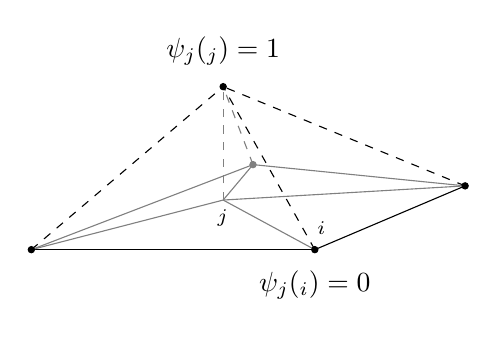
\begin{tikzpicture}[scale=0.9, z={(.707,.3)}]
    % (2,2,1) is top
    \draw[style=dashed] (0,0,0) -- (2,2,1); % to top from left
    \draw[style=dashed] (4,0,0) -- (2,2,1); %   ...  from front
    \draw[style=dashed] (4,0,3) -- (2,2,1); %   ...  from right
    \draw[color=gray, style=dashed] (0.3,0,4) -- (2,2,1); % from back
    \draw[color=gray, style=dashed] (2,0.4,1) -- (2,2,1); % from middle
    % draw base
    \draw (0,0,0) -- (4,0,0);
    \draw (4,0,0) -- (4,0,3);
    \draw[color=gray] (0,0,0) -- (0.3,0,4);
    \draw[color=gray] (0.3,0,4) -- (4,0,3);
    \draw[color=gray] (0,0,0) -- (2,0.4,1);
    \draw[color=gray] (2,0.4,1) -- (4,0,3);
    \draw[color=gray] (4,0,0) -- (2,0.4,1);
    \draw[color=gray] (2,0.4,1) -- (0.3,0,4);
    % draw \psi_j at nodes
    \filldraw (2,2,1) circle (1.25pt);
    \draw (2,2.5,1) node {$\psi_j(\bx_j)=1$};
    \draw (2,0.15,1) node {$\bx_j$};
    \filldraw (0,0,0) circle (1.25pt);
    \filldraw (4,0,0) circle (1.25pt);
    \draw (4,-0.5,0) node {$\psi_j(\bx_i)=0$};
    \draw (4.1,0.3,0) node {$\bx_i$};
    \filldraw (4,0,3) circle (1.25pt);
    \filldraw[color=gray] (0.3,0,4) circle (1.25pt);
\end{tikzpicture}


\caption{Hat functions $\psi_j$.}
\label{fig:un:hatfunction}
\end{marginfigure}

The FEM itself can now be stated.  It requires \eqref{eq:un:poissonweak} to be true for $u^h\in S_{g}^h$ for all $v^h\in S_{0}^h$.  However, it suffices to consider $v^h$ from a basis of $S_{0}^h$, so we require
\begin{equation}
\int_\Omega a(u^h) \grad u^h \cdot \grad \psi_i = \int_\Omega f(u^h) \psi_i + \int_{\partial_N\Omega} g_N \psi_i \label{eq:un:weakformhat}
\end{equation}
for all $i$ such that $\bx_i \notin \partial_D \Omega$.  On the other hand we may write $u^h$ using $N-L$ unknown coefficients $u_j\in\RR$:
\begin{equation}
u^h(x,y) = \hat g_D(x,y) + \sum_{\bx_j \notin \partial_D \Omega} u_j\, \psi_j(x,y). \label{eq:un:uhexpand}
\end{equation}
The coefficients $u_j$ are the unknowns.  The complete FEM specification of $u^h$, equivalently the vector $\bu = \{u_i\} \in \RR^{N-L}$ of coefficients, are equations \eqref{eq:un:hatgdefine}, \eqref{eq:un:weakformhat}, and \eqref{eq:un:uhexpand}.

Note that the support (i.e.~nonzero set) of $\psi_j$ includes only the node $\bx_j$ and all triangles (elements) $\triangle_k$ incident to it (i.e.~for which $\bx_j$ is a node of $\triangle_k$).  Thus the integral ``$\int_\Omega \grad \psi_j \cdot \grad \psi_i$'' in \eqref{eq:un:poissonfem} is often zero: it is zero if $\bx_i$ and $\bx_j$ are not both nodes of at least one triangle in the triangulation.  This is the property which makes \eqref{eq:un:poissonfem} a sparse system of equations, and the system matrix a sparse matrix.

Each equation in \eqref{eq:un:poissonfem} is linear.  It is therefore very common to immediately write the system \eqref{eq:un:poissonfem} as a linear equation ``$A \bu = \bb$'', but we will not do that immediately.  Following the pattern established since Chapter \ref{chap:nl}, we first implement a residual-evaluation function, corresponding to \eqref{eq:un:poissonfem}, within a \PETSc \pSNES instance.  This implementation can immediately be tested with finite-differenced Jacobian.  Once it works we can, and we will, consider matrix assembly.  Before any of that can be accomplished, however, we have to \emph{put the mesh itself into \PETSc data structures}.


\section{Triangular meshes from \Triangle}

FIXME from here: \pIS and \pSNES

\PETSc itself does not include any tools for triangulating regions of the plane, so we use the widely-available and easy-to-use \Triangle\sidenote{See \href{http://www.cs.cmu.edu/~quake/triangle.html}{www.cs.cmu.edu/$\sim$quake/ triangle.html} for documentation and source code. \Triangle may be available as a package in your operating system.} software \citep{Shewchuk1996} for this task.  \Triangle is both limited to planar regions and only capable of writing ASCII files.  Thus it is not a choice for performance, but of convenience.

\Triangle uses a simply-formatted ASCII file (extension \texttt{.poly}) as input to describe a polygonal region $\Omega$, and to indicate Dirichlet and Neumann portions of the boundary $\partial \Omega$.  FIXME For example, consider the input file \texttt{bump.poly} shown in Code \ref{code:bumppoly}.  This example polygon, a rectangle with a triangular bump in the base, is shown in Figure \ref{fig:bump-poly}.  It will reappear several times in this book as we solve more interesting PDEs on it.  The two apparently-unnecessary vertices introduced along the bottom help identify the Neumann part of the boundary, but note that \texttt{bump.poly} includes a Dirichlet/Neumann flag along each boundary segment.

\inputfromline{../c/\CODELOC/blob.poly}{\CODELOC blob.poly}{A description of the boundary polygon in Figure \ref{fig:un:polygon}, suitable for reading by \Triangle.}{8}{code:blobpoly}

The triangulation shown in Figure \ref{fig:triangulation} came from a single command which asks \Triangle to take \texttt{bump.poly} and generate a triangulation which has a polygon output file (option \texttt{-p}), relatively-uniform triangles (option \texttt{-q} for ``quality-checked'' \citep{Shewchuk1996}), and triangles with maximum area of $1.0$ (option \texttt{-a1.0}):
\begin{marginfigure}
%\input{bump.poly.tikz}
\caption{FIXME The polygon described by \texttt{bump.poly} in Code \ref{code:bumppoly}.  The bold part is the closed Dirichlet boundary.  The lower boundary is Neumann, and has ``extra'' nodes to identify it as such.}
\label{fig:bump-poly}
\end{marginfigure}
\begin{cline}
$ triangle -pqa1.0 bump
\end{cline}
%$
This command generates three ASCII files, \texttt{bump.1.poly}, \texttt{bump.1.node}, and  \texttt{bump.1.ele}.  These files define the new (i.e.~refined relative to \texttt{bump.poly}) polygonal boundary, the nodes locations, and the elements in the triangulation, respectively.

\Triangle includes a minimal visualization tool which shows the triangulation graphically.  The command
\begin{cline}
$ showme bump
\end{cline}
%$
displays the boundary polygon (from \texttt{bump.poly} or \texttt{bump.1.poly}) and the triangulation itself (\texttt{bump.1.node} and \texttt{bump.1.ele}).


\section{Getting a triangular mesh from ASCII files into a \PETSc \pVec}

The ASCII files produced by \Triangle produces are not in a good format for large meshes, but we will accept this for portability and readability.  We will, however, demonstrate how files are read in parallel, based on first doing a mundane and un-scalable task in \PETSc, namely reading the ASCII \Triangle files serially onto a single MPI process and writing out a binary file in \PETSc format.\sidenote{Furthermore we will focus on the scalability of the FEM solution process, once the mesh is loaded.}  The binary file both describes the mesh element-by-element and can be read in parallel.

The code \texttt{c3convert.c} does the conversion.  It is invoked, for the present purposes, by
\begin{cline}
$ c3convert -f bump.1
\end{cline}
%$
This reads ASCII files \texttt{bump.1.\{node,ele,poly\}} and writes a \PETSc-formatted binary file \texttt{bump.1.petsc}.

We will not show \texttt{c3convert.c}, but we summarize the high points.  First \PETSc is initialized and we obtain the rank of the current (MPI) process.  We only ask the first process (``rank zero'') in the MPI communicator to do any work.\sidenote{This code can be invoked ``\texttt{mpiexec -n NN c3convert}'', but it behaves as a serial code.}  This part of the code first reads the header information in the \texttt{.node} file, and allocates \PETSc \pVecs according.  We use \texttt{VecCreateSeq} to allocate the a sequential \pVec \texttt{vx}, which contains the $x$-coordinate of the nodes, only on the rank zero process.  Then \texttt{VecDuplicate} is used to allocate two more \pVecs with the same layout, \texttt{vy} and \texttt{vBT}.  This last \pVec will contain a flag $\{0,2,3\}$ for each node, where $0$ is an interior node, $2$ is a Dirichlet boundary node, and $3$ is a Neumann boundary node.

Then we read the node locations from the \texttt{.node} file.  The reading itself is done with the standard C library call \texttt{fscanf}.  Then \texttt{VecSetValues} is used to set one entry at a time.  After setting these values, which stores a list of entrys into an internal \PETSc dynamic data structure, we ask \PETSc to assemble the \pVecs.

The next part of \texttt{c3convert.c} reads boundary polygon information from the \texttt{.poly} file.  Each segment of the boundary polygon corresponds to two node indices.  We store the segments in a \pVec with blocksize 2.  Then we read the header information in the \texttt{.ele} file and allocates a \pVec called \texttt{vE} for the elements.  This part of the code is an important transformation of the data structures.  In fact, \texttt{vE} has block size 15,\sidenote{A \PETSc \pVec is designed to hold \texttt{double} values.  We are being quite wasteful for integer indices and boolean flags.  FIXME: A \PETSc index set \texttt{IS} should be used.} and, in contrast to the format from \Triangle, it contains all the information about each element that we need to do assemble the matrix equation.  Each of its blocks is the C \texttt{struct} shown in Code \ref{code:elementtype}.

\cinputraw{../c/\CODELOC/readmesh.h}{extract from \texttt{\CODELOC readmesh.h}}{The \texttt{elementtype} struct.}{}{//STARTSTRUCT}{//ENDSTRUCT}{code:elementtype}

In the next part of \texttt{c3convert.c} we fill the \pVec for elements with all of the information read so far, including the node indices for each element which we read from the \texttt{.ele} file.  This stage is fundamentally serial, because we must look at the entire mesh to find the node coordinates and node/segment boundary type for each node and edge of each element.  In this part there is an important detail about triangulations, which affects the data structure for elements.  Namely, we cannot tell if an edge of an element is in the boundary just by whether both endpoints are in the boundary.  For example, the element (triangle) labeled ``5'' in Figure \ref{fig:triangulation} has an edge from node 5 (on the Dirichlet boundary) to node 7 (on the Neumann boundary).  But triangle 5 is \emph{not} a boundary element.  Thus we need to have list of flags for the boundary segments themselves.  Thus the \texttt{elementtype} structure above has both a boundary type for each node of each element and a boundary type for each edge of each element.

At this point we have the entire triangulation in \PETSc \pVecs.  The almost-last part of \texttt{c3convert.c} simply creates a \PETSc ``viewer'' and ``view''\sidenote{I.e.~save to disk in \PETSc's binary format.} all of the \pVecs which contain the mesh.  We will be able to reread these \pVecs in parallel, as long as we re-read them in the same order.  The final bit of \texttt{c3convert.c} checks if option \texttt{-check} is given, and if so we read back the binary file in parallel.  This part of \texttt{c3convert.c} calls two methods from a separate code (and re-used component) \texttt{readmesh.c} (Codes \ref{code:readmeshpartone} and \ref{code:readmeshparttwo}).

The first method \texttt{getmeshfile()} finds a \PETSc binary file from the \texttt{-f} option.  The other major method \texttt{readmesh()}, in Code \ref{code:readmeshparttwo}, creates and reads three \pVecs in parallel from it, using utility methods \texttt{createloadname()} and \texttt{getcheckmeshsizes()}.  Note that prefixes are set on each \pVec so that the block size is correctly read.

\cinputpart{readmesh.c}{\CODELOC}{Determine the filename of a \PETSc binary file that has a mesh.}{I}{//STARTGET}{//ENDGET}{code:readmeshpartone}

\cinputpart{readmesh.c}{\CODELOC}{Read the mesh in parallel from the file.}{II}{//STARTREADMESH}{//ENDREADMESH}{code:readmeshparttwo}


\section{Constructing the FEM linear system}

Now that we can get a triangulation into \PETSc, we can return to the finite-dimensional weak formulation \eqref{poissonfem}.  This linear system
\begin{equation}
A \bu = \bb, \label{poissonmatrix}
\end{equation}
has $A\in\RR^{N\times N}$ and $\bu,\bb\in\RR^N$, where $N$ is the number of nodes.  We will write a code which assembles $A$ and $\bb$ and solves for $\bu$.  \PETSc \pMat and \pVec objects store the problem, and we use a \pKSP object to solve it.

For ease of construction we include the node-wise Dirichlet conditions $u_j=g(\bx_j)$ as equations in this linear system, treating such $u_j$ as unknowns, so that the matrix has $N$ rows and columns if there are $N$ nodes in total.  Thus we define $A$ to have entries
\begin{equation}
a_{ij} = \int_\Omega \grad \psi_j \cdot \grad \psi_i \label{Aentryfem}
\end{equation}
if $\bx_i \notin \partial_D \Omega$ and $\bx_j \notin \partial_D \Omega$, while otherwise
\begin{equation*}
a_{ij} = \delta_{ij}.
\end{equation*}
Notice that we index rows and columns of matrices and vectors starting with zero,\sidenote{This follows C and \PETSc conventions, but is opposed to long-standing traditions about linear algebra!} and that $j=0,1,\dots,N-1$ in particular.

Observe that $A$ is \emph{symmetric}, $a_{ij}=a_{ji}$.  Furthermore $A$ is \emph{sparse}, that is, most entries are zero, at least for triangulations with more than a handful of triangles.  These facts affect the algorithms we choose when solving \eqref{poissonmatrix}.

For the right side of \eqref{poissonfem}, define the entries
\begin{equation}
    b_i = \int_\Omega f \psi_i + \int_{\partial_N\Omega} \gamma \psi_i - \sum_{l=0,\dots,L} g(\bx_{j_l})  \int_\Omega \grad \psi_{j_l} \cdot \grad \psi_i  \label{bentryfem}
\end{equation}
if $\bx_i \notin \partial_D \Omega$, while if $\bx_i \in \partial_D \Omega$ then
    $$b_i = g(\bx_{i}).$$

In practice we \emph{don't} initially build $A$ or $\bb$ as described above.  We start with a matrix $\tilde A$ and vector $\tilde \bb$ which have the same size as $A$ and $\bb$, respectively, but which ignore the Dirichlet boundary.  We don't even evaluate the function $g$.  All entries of $\tilde A$ are computed by the first formula above for $a_{ij}$, that is, the entries are
\begin{equation*}
\tilde a_{ij} = \int_\Omega \grad \psi_i \cdot \grad \psi_j
\end{equation*}
for all $i,j=0,1,\dots,N$.  Also the simpler right-hand side $\tilde \bb\in\RR^N$ has entries
    $$\tilde b_i = \int_\Omega f \psi_i + \int_{\partial_N\Omega} \gamma \psi_i$$
for all $i=0,1,\dots,N$.

This initial linear system $\tilde A\bu=\tilde \bb$ is (obviously) final in the case where there is no Dirichlet boundary (i.e.~$\partial_D \Omega=\emptyset$).  However, in this case $u=C$, where $C\in\RR$ is any constant value, solves $-\grad^2 u=0$ with $\partial u/\partial n = 0$ on the whole boundary $\partial_N \Omega = \partial \Omega$.  The Poisson problem then only determines the solution up to such an additive constant.  Because it does not have a unique solution, when solving \eqref{poissonmatrix} in this Neumann case we will have to inform \PETSc about the null space of constant functions.

In general, the next step is to edit $\tilde A$ in each Dirichlet row, that is, for each $i$ where $\bx_i \in \partial_D \Omega$.  For each such row we replace the whole row with the corresponding row of the identity, and also we replace $\tilde b_i$ with $b_i = g(\bx_i)$.  Furthermore, in each column $j$ for which $\bx_j \in \partial_D \Omega$, we move all entries $\tilde a_{ij}$ where $i$ is \emph{not} a Dirichlet row index over to the right-hand side, multiplied by the negative of the boundary value $g(\bx_{j})$.  We can write
\begin{equation}
    \tilde b_i \to \tilde b_i - g(\bx_{j}) \tilde a_{ij} \label{btransform}
\end{equation}
for these transformations.  After the completion of this ``editing'' stage we get $A$ and $\bb$.  Since this part of the matrix assembly is a key stage in our FEM codes, we now give a concrete example.

\medskip\noindent\hrulefill
\begin{example} Figure \ref{fig:squarefour} shows a triangulation of the unit square with five nodes.  The matrix $\tilde A$ has the following nonzero pattern; the zero entries are shown as spaces:\begin{marginfigure}
\input{tmp/squarefour.tikz}
\caption{A triangulation of a square with five nodes.  The top segment is the Dirichlet boundary.}
\label{fig:squarefour}
\end{marginfigure}%
\begin{equation*}
\tilde A = \begin{bmatrix}
\X & \X &    & \X & \X \\
\X & \X & \X &    & \X \\
   & \X & \X & \X & \X \\
\X &    & \X & \X & \X \\
\X & \X & \X & \X & \X
\end{bmatrix}.
\end{equation*}
Note $\tilde a_{ij}=0$ only where the integral $\int_\Omega \grad \psi_j \cdot \grad \psi_i$ is zero, a rare event in this small (coarse)-mesh case.  Now, because the $i=1,2$ nodes live in the (closed) Dirichlet boundary $\partial_D \Omega$, we highlight the $i=1,2$ rows and $j=1,2$ columns which will be edited:\marginnote{\emph{Caution}:  The first row or column of any matrix in this book is numbered ``$0$.''}

\newcommand{\uX}{\underline{\X}}
\newcommand{\hX}{\widehat{\X}}

\begin{equation*}
\tilde A = \begin{bmatrix}
\X  & \hX &     & \X  & \X \\
\uX & \uX & \uX &     & \uX \\
    & \uX & \uX & \uX & \uX \\
\X  &     & \hX & \X  & \X \\
\X  & \hX & \hX & \X  & \X
\end{bmatrix}.
\end{equation*}
The underlined entries ``$\uX$'' are changed to $0$ or $1$ so that these rows become rows of the identity; the old computed values $\tilde a_{ij}$ are tossed out.  The hatted entries ``$\hX$'', specifically the four entries $\tilde a_{01}$, $\tilde a_{32}$, $\tilde a_{41}$, and $\tilde a_{42}$, are moved over to the right side using transformation \eqref{btransform}; these $\tilde a_{ij}$ values get used.  The final linear system $A \bu = \bb$, is
\begin{equation*}
\begin{bmatrix}
\X & & & \X & \X \\
 & \,1\, & & & \\
 & & \,1\, & & \\
\X & & & \X & \X \\
\X & & & \X & \X
\end{bmatrix}
\begin{bmatrix}
u_0 \\
u_1 \\
u_2 \\
u_3 \\
u_4
\end{bmatrix}
=
\begin{bmatrix}
\tilde b_0 - g(\bx_1) \tilde a_{01} \\
g(\bx_1) \\
g(\bx_2) \\
\tilde b_3 - g(\bx_2) \tilde a_{32} \\
\tilde b_4 - g(\bx_1) \tilde a_{41} - g(\bx_2) \tilde a_{42}
\end{bmatrix}
\end{equation*}
\end{example}
\noindent\hrulefill

\bigskip


\section{Assembling the matrix equation, element by element}

An entry $\tilde a_{ij}$ of the initial matrix $\tilde A$ is not computed in one step.  Rather, we compute contributions to these entries from each element in turn; we ``loop over the elements.''  Furthermore we do it in parallel.  Recall that \texttt{c3convert.c} above creates a distributed \pVec called \texttt{E}, which is an array of elements of type \texttt{elementtype}, and \texttt{readmesh.c} reads it.

For the element-by-element assembly procedure we first define the integral over one triangle $\triangle_k$,
\begin{equation}
\text{\texttt{a(k,i,j)}} = \int_{\triangle_k} \grad \psi_i \cdot \grad \psi_. \label{aelementintegral}
\end{equation}
so that
    $$\tilde a_{ij} = \sum_k \phantom{.}\text{\texttt{a(k,i,j)}}.$$
Likewise we will compute
\begin{equation}
\text{\texttt{b(k,i)}} = \int_{\triangle_k} f \psi_i + \int_{\overline{\triangle}_k \cap \partial_N\Omega} \gamma \psi_i, \label{belementintegral}
\end{equation}
so that $\tilde b_i = \sum_{k} \;\text{\texttt{b(k,i)}}$.

If \texttt{E} denotes an array of \texttt{elementtype} then for each triangle $\triangle_k$ we can get the node index for each of its three vertices.  Using $q=0,1,2$ for these vertices,
    $$\text{\texttt{E[k].j[q]}} \in \{0,1,\dots,N-1\}.$$
Thus the element-by-element assembly of $\tilde A$ follows this pseudocode:
\begin{code}
A = 0                           // N x N sparse matrix with entries a(i,j)
b = 0                           // N x 1 column vector with entries b(i)
for k = 0 to K-1                // loop through all elements
    for q = 0 to 2
        i = E[k].j[q]           // row index
        for r = 0 to 2
            j = E[k].j[r]       // column index
            a(i,j) += a(k,q,r)  // add contribution from element k
            b(i)   += b(k,q)    // ditto
\end{code}
\medskip\noindent
Observe that on each triangle $\triangle_k$ we write ``\texttt{a(k,q,r)}'' for \texttt{a(k,i,j)}, by replacing the global indices $i,j$ by corresponding local node indices $q,r\in\{0,1,2\}$ for triangle $k$.

A standard approach to computing the element-wise integrals \texttt{a(k,q,r)} is to refer triangle $\triangle_k$ to a reference triangle $\triangle_\ast$ with vertices $(0,0),\,(1,0),\,(0,1)$, as shown in Figure \ref{fig:isoparametric}.  The linear map from $\triangle_\ast$ to $\triangle_k$ with vertices $(x_0,y_0),\,(x_1,y_1),\,(x_2,y_2)$, as shown in the Figure, is
\begin{align}
x(\xi,\eta) &= x_0 + (x_1-x_0) \xi + (x_2-x_0) \eta, \label{trianglemap} \\
y(\xi,\eta) &= y_0 + (y_1-y_0) \xi + (y_2-y_0) \eta. \notag
\end{align}

\begin{marginfigure}
\begin{tikzpicture}[scale=1.1,
    decoration={
      markings,
      mark=at position 1 with {\arrow[scale=1.8,gray]{latex}};
    }]
% left x,y axes
    \draw[->, gray, very thin] (1.5,0) -- (4.0,0);
    \draw[->, gray, very thin] (2,-0.5) -- (2,2.4);
    \draw (4.1,-0.1) node {$x$};
    \draw (1.9,2.4) node {$y$};
    \filldraw (1.7,1) circle (1.25pt);    % (x_0,y_0)
    \filldraw (3.5,-0.3) circle (1.25pt); % (x_1,y_1)
    \filldraw (3.0,2.0) circle (1.25pt);  % (x_2,y_2)
    \draw (1.4,1.3) node {$(x_0,y_0)$};
    \draw (3.5,-0.6) node {$(x_1,y_1)$};
    \draw (3.0,2.3) node {$(x_2,y_2)$};
    \draw[line width=1pt] (1.7,1) -- (3.5,-0.3) -- (3.0,2.0) -- cycle;
    \draw (2.7,1.0) node {$\triangle_k$};
% right xi,eta axes
    \draw[->, gray, very thin] (4.6,0) -- (6.6,0);
    \draw[->, gray, very thin] (5,-0.4) -- (5,2.0);
    \draw (6.7,-0.1) node {$\xi$};
    \draw (4.9,2.05) node {$\eta$};
    \filldraw (5,0) circle (1.25pt);  % (0,0)
    \filldraw (6,0) circle (1.25pt);  % (1,0)
    \filldraw (5,1) circle (1.25pt);  % (0,1)
    \draw (5.2,-0.3) node {$0$};
    \draw (6.2,0.2) node {$1$};
    \draw (5.2,1.1) node {$2$};
    \draw[line width=1pt] (5,0) -- (6,0) -- (5,1) -- cycle;
    \draw (5.3,0.3) node {$\triangle_\ast$};
% arrows connecting nodes
    \draw[gray, postaction={decorate}] (5,0) -- (1.7,1.03);
    \draw[gray, postaction={decorate}] (6,0) -- (3.5,-0.3);
    \draw[gray, postaction={decorate}] (5,1) -- (3.0,2.0);
\end{tikzpicture}


\caption{Mapping of a triangle $\triangle_k$ from the reference triangle $\triangle_\ast$.}
\label{fig:isoparametric}
\end{marginfigure}

\noindent Furthermore, on $\triangle_\ast$ any linear function is a linear combination of these three local basis functions:
\begin{equation}
\chi_0(\xi,\eta) = 1-\xi-\eta, \qquad \chi_1(\xi,\eta) = \xi, \qquad \chi_2(\xi,\eta) = \eta. \label{chiformulas}
\end{equation}
On $\triangle_k$, each of the basis functions $\psi_q$ is the mapped version of the corresponding $\chi_q$:
\begin{equation}
\psi_q(x(\xi,\eta),y(\xi,\eta)) = \chi_q(\xi,\eta). \label{phichimap}
\end{equation}
From \eqref{trianglemap} and \eqref{phichimap} one can confirm that $\psi_q(x_r,y_r) = \delta_{qr}$.

Now is a good point at which to observe that the set of $\psi_j$, over all nodes $j=0,1,\dots,N$, is a partition of unity.  We can see this by switching to local node coordinate $q$ and using $\chi_0+\chi_1+\chi_2=1$, which is obvious from \eqref{chiformulas}.  That is, if $\bx \in \triangle_k$ then
\begin{equation}
   \sum_j \psi_j(\bx) = \sum_{q=0,1,2} \psi_q(\bx) = \sum_{q=0,1,2} \chi_q =1.  \label{partitionofunity}
\end{equation}

The Jacobian\sidenote{By definition, the \emph{Jacobian} $J=J(\bx)$ of a smooth map $F$ at a point $\bx$ is its linearization at $\bx$.  That is, if $\by=F(\bx)$ and $\by+\Delta\by = F(\bx+\Delta\bx)$ then $J(\bx)$ satisfies $\Delta \by = J(\bx) \Delta\bx + o(|\Delta\bx|)$.} of map \eqref{trianglemap} is
% CAUTION: Elman (1.37) uses "Jacobian" for the transpose of this, the true Jacobian (e.g. in Newton later)
\begin{equation}
J = \begin{bmatrix}
    \dfrac{\partial x}{\partial \xi} & \dfrac{\partial x}{\partial \eta} \\[1.0em]
    \dfrac{\partial y}{\partial \xi} & \dfrac{\partial y}{\partial \eta}
    \end{bmatrix}
    =
    \begin{bmatrix}
    x_1-x_0 & x_2-x_0 \\
    y_1-y_0 & y_2-y_0
    \end{bmatrix}.  \label{trianglejacobian}
\end{equation}
Recalling both the change-of-variables formula for integrals\sidenote{If $F$ is a smooth map from $\bx \in U$ to $\by \in F(U)$, $J$ is the Jacobian of $F$, and $g$ is integrable on $F(U)$, then $$\int_{F(U)} g(\by)\,d\by = \int_U g(F(\bx))\,|\det(J)|\,d\bx.$$} and the chain rule, by \eqref{phichimap} we can write
\begin{align}
\text{\texttt{a(k,q,r)}} &= \int_{\triangle_k} \grad\psi_q \cdot \grad\psi_r \label{elementcontrib} \\
   &= \int_{\triangle_k} \frac{\partial\psi_q}{\partial x} \frac{\partial\psi_r}{\partial x} + \frac{\partial\psi_q}{\partial y} \frac{\partial\psi_r}{\partial y} \; dx \, dy  \notag \\
   &= \int_{\triangle_\ast} \left(\frac{\partial \chi_q}{\partial \xi} \frac{\partial \xi}{\partial x} + \frac{\partial \chi_q}{\partial \eta} \frac{\partial \eta}{\partial x}\right) \left(\frac{\partial \chi_r}{\partial \xi} \frac{\partial \xi}{\partial x} + \frac{\partial \chi_r}{\partial \eta} \frac{\partial \eta}{\partial x}\right) \notag \\
   &\qquad\qquad + \left(\frac{\partial \chi_q}{\partial \xi} \frac{\partial \xi}{\partial y} + \frac{\partial \chi_q}{\partial \eta} \frac{\partial \eta}{\partial y}\right) \left(\frac{\partial \chi_r}{\partial \xi} \frac{\partial \xi}{\partial y} + \frac{\partial \chi_r}{\partial \eta} \frac{\partial \eta}{\partial y}\right) \; |\det(J)| \; d\xi \, d\eta. \notag
\end{align}
The last expression is the low point of this calculation.  From now on the formulas simplify because the integrand is \emph{constant} for the $\Pone$ elements here.  Indeed, by \eqref{trianglejacobian} we see $\det(J)$ is constant, but also the derivatives $\partial \chi_q/\partial\{\xi,\eta\}$ and $\partial\{\xi,\eta\}/\partial\{x,y\}$ are all constant because the functions in question are linear.

However, we need computable formulas for ``$\partial \xi/\partial x$'' and similar terms.  Again by the chain rule we can compute
\begin{equation*}
\begin{bmatrix}
    1 & 0 \\[0.2em]
    0 & 1
\end{bmatrix}
=\begin{bmatrix}
    \dfrac{\partial x}{\partial x} & \dfrac{\partial x}{\partial y} \\[1.0em]
    \dfrac{\partial y}{\partial x} & \dfrac{\partial y}{\partial y}
\end{bmatrix}
=
\begin{bmatrix}
    \dfrac{\partial x}{\partial \xi} & \dfrac{\partial x}{\partial \eta} \\[1.0em]
    \dfrac{\partial y}{\partial \xi} & \dfrac{\partial y}{\partial \eta}
\end{bmatrix}
\begin{bmatrix}
    \dfrac{\partial \xi}{\partial x} & \dfrac{\partial \xi}{\partial y} \\[1.0em]
    \dfrac{\partial \eta}{\partial x} & \dfrac{\partial \eta}{\partial y}
\end{bmatrix},
\end{equation*}
which is to say $I=J\; J^{-1}$.  On the other hand we can invert the $2\times 2$ matrix $J$ by hand to get
\begin{equation}
J^{-1}
= \frac{1}{\det(J)}
\begin{bmatrix}
    \dfrac{\partial y}{\partial \eta} & -\dfrac{\partial x}{\partial \eta} \\[1.0em]
    -\dfrac{\partial y}{\partial \xi} & \dfrac{\partial x}{\partial \xi}
\end{bmatrix}
= \frac{1}{\det(J)}
\begin{bmatrix}
    y_2-y_0 & x_0-x_2 \\
    y_0-y_1 & x_1-x_0
\end{bmatrix}.  \label{Jinverse}
\end{equation}
Now let $y_{20}=y_2-y_0$, $x_{02}=x_0-x_2$, $y_{01}=y_0-y_1$ and $x_{10}=x_1-x_0$.  In terms of these differences,
\begin{equation}
\begin{bmatrix}
    \dfrac{\partial \xi}{\partial x} & \dfrac{\partial \xi}{\partial y} \\[1.0em]
    \dfrac{\partial \eta}{\partial x} & \dfrac{\partial \eta}{\partial y}
\end{bmatrix}
= \frac{1}{\det(J)}
\begin{bmatrix}
    y_{20} & x_{02} \\
    y_{01} & x_{10}
\end{bmatrix} \label{dxietadxy}
\end{equation}
and
\begin{equation}
\det(J) = x_{10} y_{20} - y_{01} x_{02}. \label{detJ}
\end{equation}
Thus, by \eqref{elementcontrib}, \eqref{dxietadxy}, and \eqref{detJ}, and because the area of the reference triangle $\triangle_\ast$ is $1/2$\,, our element-wise contribution to $\tilde a_{ij}$ simplifies to
\begin{align}
\text{\texttt{a(k,q,r)}} = \frac{1}{2\; |\det(J)|} &\bigg[\left(\frac{\partial \chi_q}{\partial \xi} y_{20} + \frac{\partial \chi_q}{\partial \eta} y_{01}\right) \left(\frac{\partial \chi_r}{\partial \xi} y_{20} + \frac{\partial \chi_r}{\partial \eta} y_{01}\right) \label{elementcontribFINAL} \\
&\quad + \left(\frac{\partial \chi_q}{\partial \xi} x_{02} + \frac{\partial \chi_q}{\partial \eta} x_{10}\right) \left(\frac{\partial \chi_r}{\partial \xi} x_{02} + \frac{\partial \chi_r}{\partial \eta} x_{10}\right)\bigg]. \notag
\end{align}
Also note that
\begin{align}
\frac{\partial \chi_0}{\partial \xi} &= -1, & \frac{\partial \chi_1}{\partial \xi} &= 1, & \frac{\partial \chi_2}{\partial \xi} &= 0, \label{chiderivs} \\
\frac{\partial \chi_0}{\partial \eta} &= -1, & \frac{\partial \chi_1}{\partial \eta} &= 0, & \frac{\partial \chi_2}{\partial \eta} &= 1. \notag
\end{align}
Combining \eqref{elementcontribFINAL} and \eqref{chiderivs}, we know enough to write code to compute \texttt{a(k,q,r)}, and thus the entries in $\tilde A$.

To complete the code for the initial linear system $\tilde A \bu = \tilde\bb$ we also need to address the right-hand side $\tilde\bb$, that is, we need to compute the element-wise contribution \texttt{b(k,i)} in \eqref{belementintegral}.  We do these integrals by changing variables to the reference element, but we also only do the integrals approximately by quadrature.  This is because the data $f$ and $\gamma$ may have no analytically-computable integral, and because a modest error in evaluating the right side of the linear system can have only a small effect on the solution of the FEM linear system, which is, after all, only an approximation of the solution of the Poisson problem.

FIXME: in the homogeneous Neumann case ($\gamma=0$) we use midpoints of the edges of the triangles in our quadrature rule from \citet{Ciarlet2002}
\begin{align*}
\text{\texttt{b(k,q)}} &= \int_{\triangle_\ast} f\, \chi_q \; |\det(J)| \; d\xi \, d\eta \\
  &\approx \frac{|\det(J)|}{6} \left(\omega(0.5,0) + \omega(0.5,0.5) + \omega(0,0.5)\right)
\end{align*}
where $\omega(\xi,\eta) = f(x(\xi,\eta),y(\xi,\eta)) \chi_q(\xi,\eta)$.

%\section{Preallocate a \pMat}
%FIXME: figure showing parallel partition of elements
%\cinputpart{testprealloc.c}{Read mesh \pVecs from file.  Get row ownership range.}{I}{//STARTLOAD}{//ENDLOAD}{code:testpreallocpartone}
%\cinputpart{testprealloc.c}{Set up \pMat $A$ and actually preallocate it.  Fill it with junk entries so the pattern can be visualized.}{II}{//ENDLOAD}{//ENDTEST}{code:testpreallocparttwo}

\begin{comment}
From: Fande Kong <fdkong.jd@gmail.com>
To: PETSc users list <petsc-users@mcs.anl.gov>
Subject: Re: [petsc-users] Status on parallel mesh reader in DMPlex
> Message: 2
>Date: Fri, 18 Dec 2015 08:21:04 -0800
>From: Justin Chang <jychang48@gmail.com>
>To: petsc-users <petsc-users@mcs.anl.gov>
>Subject: [petsc-users] Status on parallel mesh reader in DMPlex

> Hi all,

>What's the status on the implementation of the parallel

I am actually developing a parallel loader. The loader has two steps:

(1) Use 1 core or several cores to read a sequential  mesh, and partition
it into $np$ parts using a partitioner, $np$ is the number of cores you
want to use to do a simulation. Usually, $np$ is large, for example, 10,000
cores. And then we write the partitioned data into the file system as a
HDF5 file.

(2) Load the partitioned data (HDF5 file) into $np$ cores in parallel.

This idea works pretty well for me at this point.  But, this loader is
not compatible with DMPlex now. However, I could change the code somehow,
If this idea is acceptable.

You could also implement it by yourself. It is not too bad.

>mesh reader/generator for DMPlex meshes? Is anyone actively working on
> this? If so is there a branch that I can peek into?

Parallel generator is highly nontrivial, I think. It is a very hard topic.

> Thanks,
> Justin
\end{comment}


\section{Solve the Poisson problem}

\cinputpart{poissontools.c}{\CODELOC}{Find Dirichlet rows, \texttt{INSERT\_VALUES} these, and call \texttt{MatAssemblyBegin/End} and \texttt{VecAssemblyBegin/End}.}{I}{//DIRICHLETROWS}{//ENDDIRICHLETROWS}{code:poissontoolsdirichlet}

\cinputpart{poissontools.c}{\CODELOC}{Start computing all other contributions element-by-element: Precompute all geometry of element and quadrature points.}{II}{//ASSEMBLEADDONE}{//ENDONE}{code:poissontoolsaddone}

\cinputpart{poissontools.c}{\CODELOC}{Compute all other contributions element-by-element including source $f$, Dirichlet columns using data $g$, and Neumann data $\gamma$.  Use \texttt{ADD\_VALUES} for these, and call \texttt{MatAssemblyBegin/End} and \texttt{VecAssemblyBegin/End}.}{III}{//ENDONE}{//ENDASSEMBLEADD}{code:poissontoolsaddtwo}

\cinputpart{poissontools.c}{\CODELOC}{Call \texttt{dirichletrows()} and \texttt{assembleadd()}.}{IV}{//FULLASSEMBLE}{//ENDFULLASSEMBLE}{code:poissontoolsassemble}


\cinputpart{poissonfem.c}{\CODELOC}{Read in mesh in parallel (i.e.~\pVec \texttt{E}) and create \pMat \texttt{A} and \pVec \texttt{b}.}{I}{//GETMESH}{//ENDMATVECCREATE}{code:cthreepoissongetmesh}

In the next part of the code (Code \ref{code:cthreepoissonchecks}) we do two basic checks on our assembly procedure, without solving a linear system.  First we check the construction of \texttt{A} by checking if constant functions are in the kernel when $\partial_D\Omega=\emptyset$.  In this check the data $f$, $g$, and $\gamma$ are all not used, and the boundary information in \texttt{E} is not used either.

\cinputpart{poissonfem.c}{\CODELOC}{Do two checks on the construction of the linear system.}{II}{//TWOCHECKS}{//ENDTWOCHECKS}{code:cthreepoissonchecks}

In the second check we verify the construction of $\bb$ in the case where $f\equiv 1$, $\gamma=0$, and $\partial_D\Omega=\emptyset$.  In this case, by formula \eqref{bentryfem} and observation \eqref{partitionofunity}, the sum of the entries of $\bb$ should be the area of the region:
   $$\sum_j b_j = \sum_j \int_\Omega 1\, \psi_j = \int_\Omega \sum_j \psi_j = |\Omega|.$$

\cinputpart{poissonfem.c}{\CODELOC}{Solve a Dirichlet problem for which we know the solution.}{III}{//SOLVEMANU}{//ENDSOLVEMANU}{code:cthreepoissonsolvemanu}


%\caveat{It works, but does it work well?}
